\documentclass[
    english,
    accentcolor=9c,
    design=2023,
    logofile=images/hulogo.pdf,
]{tudabeamer}

\usepackage[english]{babel}
\usepackage[autostyle]{csquotes}
\usepackage{bookmark}
\newcommand*{\code}[1]{\texttt{#1}}

\title[LikertShift]{LikertShift - An Input Device for Recording Cycling Subjective Experiences}
\subtitle{Bachelor's Thesis Defense}
\author{Max Schlecht}
\department{Human Computer Interaction}
\institute{Humboldt-Universität zu Berlin}

\date{2025-08-13}

\AtBeginSection{\sectionpage} % Enable section pages

\makeatletter
\patchcmd{\beamer@sectionintoc}
{\vfill}
{\vskip\itemsep}
{}
{}
\makeatother

\let\footnoterule\relax
\renewcommand\thefootnote{}
\setbeamerfont{footnote}{size=\tiny}

\begin{document}

\maketitle

\tableofcontents

\section{Motivation}

\begin{frame}{Motivation}
    \centering
    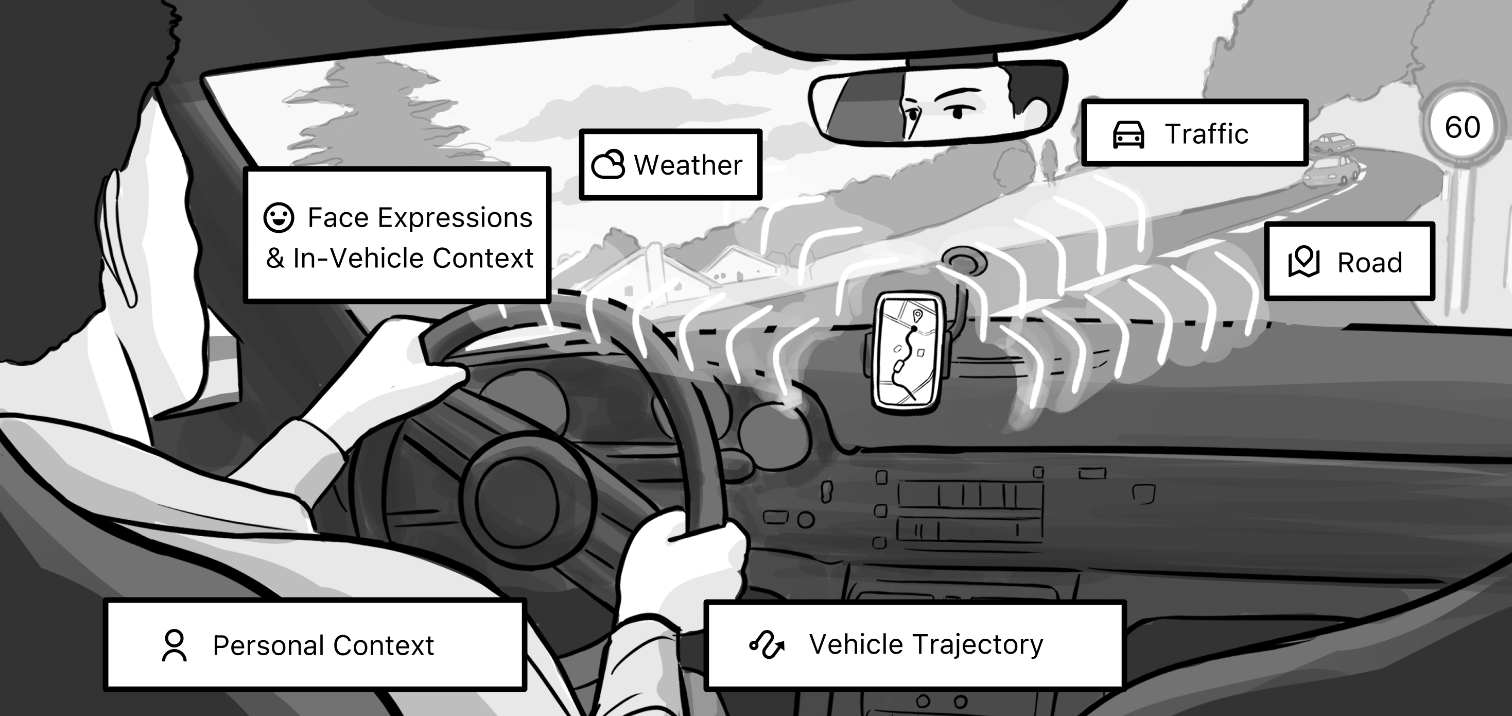
\includegraphics[height=0.35\linewidth]{images/vemotion.png}
    \footnotetext{VEmotion (Bethge et al.) \quad \url{https://doi.org/10.1145/3472749.3474775}}
\end{frame}

\begin{frame}{Motivation}
    \begin{columns}[onlytextwidth,c]
        \column{.5\linewidth}
        \centering
        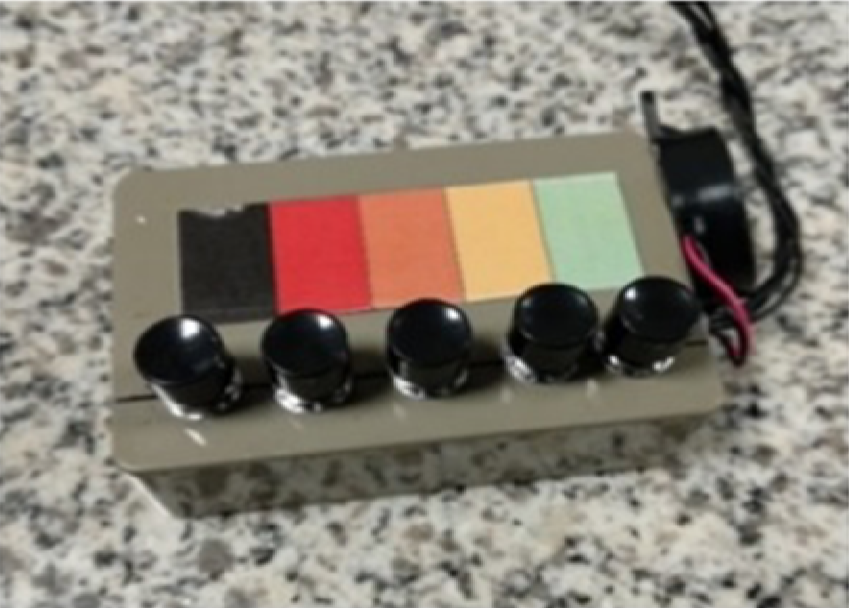
\includegraphics[height=0.55\linewidth]{images/button_device.png}
        \footnotetext{Analysis of Overtaking Maneuvers \ldots (L\'{o}pez et al.)}
        \footnotetext{\url{https://doi.org/10.1145/3472749.3474775}}
        \column{.5\linewidth}
        \centering
        \includegraphics<2>[height=0.55\linewidth]{images/brotate.png}
        \footnotetext<2>{Brotate and Tribike \ldots (Wo\'{z}niak et al.)}
        \footnotetext<2>{\url{https://doi.org/10.1145/3472749.3474775}}
    \end{columns}
\end{frame}


\end{document}
